% Working Chapter 2, 2026-10-24. Source/evidence records: planning/verification-background.md.
% HyperKG evidence uses the author's confirmed publication-equivalent arXiv PDF.
\chapter{Background and Related Work}
\label{ch:background}

This chapter reviews knowledge structures for language-model understanding and reasoning. We begin with knowledge-enhanced table annotation, then examine graph construction from task data and retrieval-based adaptation. Multimodal retrieval and context processing extend this direction to text and images. Section~\ref{sec:background:hyperkg} presents our study of information preservation in hyper-relational knowledge graphs.

\section{Knowledge Graphs and Language Models}
\label{sec:background:knowledge-models}

A knowledge graph represents entities and their relationships explicitly. In a conventional relational representation, a fact is a triple $(s,r,o)$, where $s$ is a subject entity, $r$ a relation, and $o$ an object entity. A set of these facts forms a directed graph whose edge labels identify relations. Wikidata provides a collaborative knowledge resource in which structured statements and their qualifiers can describe entities beyond the content of a single document~\cite{bg-wikidata}. A model accessing this graph can retrieve relations associated with a mentioned entity, including information absent from its immediate input.

The graph representation separates an entity's identity from the strings used to mention it. A table cell or query contains a mention, while an entity node refers to an indexed object. Entity linking establishes a correspondence between the two. A short name may match several entities, so a retrieval score and a contextual disambiguation rule can influence which facts become available. When a graph is extracted from text, repeated strings, aliases, and synonyms affect whether different passages share a node. These indexing choices determine possible paths before a query-specific selection algorithm begins.

Graph neighborhoods, paths, and subgraphs support different retrieval operations. Neighborhood aggregation enriches entity representations. Paths connect entities mentioned in a question. Subgraphs collect several relevant facts and their relationships. The edge type determines how a connection should be interpreted, whether it represents a fact, lexical similarity, or a keyword--label association.

Language models provide a complementary representation. The Transformer uses attention to compute token representations from their context~\cite{bg-transformer}. BERT pre-trains bidirectional contextual representations and can be fine-tuned with a task-specific output layer~\cite{bg-bert}. In column annotation, contextual token vectors can represent a column and feed a classifier. Generative language models produce an answer sequence conditioned on the query and supplied context.

Fine-tuning modifies model parameters using labeled examples. Retrieval supplies evidence from an external index at prediction time. KGLink fine-tunes an annotation model with graph-derived inputs. The later chapters study retrieval-based adaptation, which incorporates new task evidence while keeping model parameters fixed.

\section{Knowledge-enhanced Table Understanding}
\label{sec:background:tables}

Column-type annotation assigns semantic labels to table columns. Similar values can require different labels under different annotation vocabularies. A column of people may be labeled Name or assigned an occupation category. Surrounding columns and external facts can help determine the intended type.

Sherlock trains a neural type detector from statistical properties, character distributions, word embeddings, and paragraph vectors~\cite{bg-sherlock}. Sato adds topic features and structured prediction to model which column types occur together~\cite{bg-sato}. The two approaches differ in whether table context contributes to the prediction.

Doduo serializes multiple columns for a pre-trained language model and learns column-type and column-property annotations from their contextual representations~\cite{bg-doduo}. Self-attention lets a column representation depend on values in other columns, subject to the input-length limit.

Knowledge-based methods obtain evidence through a different route. HNN combines learned table features with knowledge-base lookup and inter-column semantics~\cite{bg-hnn}. A knowledge resource can identify a relation between mentioned objects that the table's strings do not explain. RECA uses related tables as an additional contextual source~\cite{bg-reca}. These approaches extend the information available within the target table through external semantic facts or evidence from other tables. Their retrieval units and preparation costs differ accordingly.

KGLink retrieves candidate entities for cell mentions and filters them through connections between columns~\cite{bg-kglink}. Candidate-type text and a separate KG feature sequence enrich the column representation. A contextual type-representation objective learns the correspondence between graph descriptions and annotation labels. Chapter~\ref{ch:kglink} presents the method and experiments.

These methods obtain context from different sources. Statistical features summarize column contents, contextual encoders model values jointly, RECA retrieves related tables, and knowledge-based methods retrieve external facts. Their coverage determines which ambiguities they can resolve.

\section{Retrieval-augmented Generation}
\label{sec:background:rag}

Retrieval-augmented generation conditions a generative model on information selected from an external collection~\cite{bg-rag}. A retrieval stage maps the query to indexed evidence, and a generation stage uses the evidence to produce an answer. The distinction makes the external collection an explicit part of the prediction system. Changing its contents or its selection rule changes the context received by the generator even when the generator's parameters stay fixed.

A passage-based RAG pipeline divides a corpus into chunks, indexes them, and concatenates the retrieved chunks with the query. Small chunks can separate a fact from its explanation. Large chunks preserve more context but consume more input tokens. Overlap retains information across chunk boundaries at the cost of repeating some text.

Sparse retrieval scores lexical evidence. BM25 combines within-document term frequency with corpus frequency and document-length normalization~\cite{bg-bm25}. It distinguishes a query term that occurs widely from one that is concentrated in fewer indexed items. Dense retrieval instead represents queries and passages as vectors and scores their correspondence in a learned space. Dense Passage Retrieval uses a dual-encoder framework with separate question and passage encoders~\cite{bg-dpr}. The two representations provide different signals, so hybrid retrieval can select context using both lexical overlap and embedding similarity.

For a query $q$ and indexed evidence item $e$, write the retrieval score abstractly as $s(q,e)$. A conventional fixed-budget result contains the highest-scoring $k$ items. Evidence is scored at the chosen item granularity, and the retrieval cutoff controls how many items are returned. A graph-based system can alter either assumption. It can score relationships as well as items, or determine the context by a structural condition such as connecting query anchors. The resulting context is then a selected relational object with a serialization for the language model.

Retrieval evaluation measures whether the selected context contains supporting evidence. Generation evaluation measures the resulting answer through correctness, reference overlap, or model-based assessment. An answer improvement can arise from selecting better evidence, organizing the context, or using it more effectively.

An evolving collection adds a maintenance problem. Newly available documents, examples, or labels must enter the index before retrieval can use them. Updating stored evidence can involve new embeddings, new graph nodes, changed edge weights, or derived summaries. The information supplied by an update also matters. A labeled support example carries a provided class, while a query processed online may carry only a model prediction. GORAG makes this distinction part of its dynamic classification protocol~\cite{bg-gorag}. Its index expands as observations arrive, and retrieval uses the graph state available at the current prediction.

Retrieving more passages can increase both answer coverage and model-processing cost. The retrieval budget therefore affects the information available to the generator even when the corpus and model remain fixed.

The indexed object can differ from the retrieved context. A document can contribute several graph facts, a traversal can return candidate labels, and a prompt can combine selected relationships with source passages. Graph retrieval makes these connections available during evidence selection.

\section{Graph-based Evidence Retrieval}
\label{sec:background:graph-retrieval}

Graph indexes connect entities, passages, labels, and other evidence items through extracted facts, shared mentions, or semantic similarity. Retrieval selects the nodes and connections relevant to the current query.

GraphRAG builds an entity graph and community summaries for query-focused summarization~\cite{bg-graphrag}. Community summaries provide a retrieval unit above individual passages and support questions about broader corpus themes.

HippoRAG combines language-model extraction, a knowledge graph, and personalized PageRank~\cite{bg-hipporag}. Query entities seed propagation through the graph, producing a ranking of related evidence. This ranking does not require all selected nodes to belong to one terminal-connecting structure.

LightRAG combines graph and vector representations, low- and high-level retrieval, and incremental index updates~\cite{bg-lightrag}. Its retrieval modes select specific entity information and broader relational or conceptual information.

Table~\ref{tab:background:retrieval-units} compares the evidence organization of these approaches with passage retrieval. It identifies the evidence object made available to each retrieval computation.

\begin{table}[tbp]
\centering
\caption{Representative retrieval organizations and the evidence structures they expose. Each row refers to the cited method's design.}
\label{tab:background:retrieval-units}
\small
\begin{tabular}{p{0.20\linewidth}p{0.32\linewidth}p{0.36\linewidth}}
\toprule
Method&Indexed representation&Query-related retrieval operation\\
\midrule
DPR~\cite{bg-dpr}&Dense passage representations&Question--passage similarity scoring\\
GraphRAG~\cite{bg-graphrag}&Entity graph and community summaries&Use of graph-derived summaries for query-focused summarization\\
HippoRAG~\cite{bg-hipporag}&Knowledge graph linked to passages&Personalized PageRank from query-related entities\\
LightRAG~\cite{bg-lightrag}&Graph and vector representations&Dual-level retrieval of specific and broader information\\
\bottomrule
\end{tabular}
\end{table}

Personalized propagation ranks evidence by influence from query anchors. Terminal-connecting retrieval instead selects paths that include a specified set of nodes, admitting intermediate nodes when needed. The former locates relevant graph regions; the latter constructs connections among required evidence items.

A graph result must be converted into model input. Entity retrieval requires finding associated source passages. Path retrieval requires serializing entities and relations. Community retrieval can return derived summaries. These choices determine which original details and relationships remain available to generation.

Our research moves from retrieving candidate classes to retrieving facts that support an answer. GORAG constructs a task graph and retrieves labels by connecting keywords extracted from the query~\cite{bg-gorag}. AGRAG selects connected textual evidence while considering node influence and edge cost~\cite{bg-agrag}. MGRAG constructs query-related multimodal graphs and matches query relations to semantic paths~\cite{bg-mgrag}. A set of highly ranked nodes need not contain paths connecting the requested facts, while intermediate nodes can supply useful relationships even when their direct query similarity is lower.

Passage nodes link extracted relations to their original wording. Combining graph serialization with source chunks gives the generator both connected facts and surrounding context. AGRAG uses this combination for text, and MGRAG retains source chunks containing the original images.

\section{Multimodal Retrieval and Context Serving}
\label{sec:background:multimodal}

Multimodal question answering requires evidence represented in more than one modality. MultiModalQA includes questions over text, tables, and images and studies combinations of evidence across them~\cite{bg-mmqa}. The evidence needed for a question can occur in different source objects. A relationship stated in text may identify the image whose visual content contains the answer. Retrieval must therefore consider both the relevance of individual objects and the relationship connecting them to the question.

Images can be ranked through captions or visual embeddings. Captions expose selected visual content in a text embedding space, while the original images preserve details for multimodal generation. MGRAG ranks images through captions and supplies selected original chunks to the answering model~\cite{bg-mgrag}.

MRAMG-Bench studies retrieval-augmented generation in which answers can combine text and images~\cite{bg-mramg}. Its multimodal output requirement adds another distinction between finding supporting evidence and presenting the response. The MGRAG evaluation uses six MRAMG subsets together with MMQA. Chapter~\ref{ch:mgrag} specifies the retrieval and answer-assessment protocol used for these datasets.

Once evidence is retrieved, the system must process it as model context. In an autoregressive Transformer, the prefill stage computes representations for the supplied input, and decoding generates answer tokens. Key and value tensors from processed input positions can be cached for later attention computation~\cite{bg-transformer,bg-cacheblend}. Reusing these tensors concerns the computation associated with selected evidence. It is a separate decision from choosing which evidence belongs in the context.

CacheGen addresses the storage and transfer of context caches through compression and streaming~\cite{bg-cachegen}. The relevant resource includes the cost of fetching cached tensors as well as computing context representations. CacheBlend studies combining precomputed caches for several chunks by selectively recomputing part of their key and value states~\cite{bg-cacheblend}. Its motivation includes interactions between chunks that were not present when their caches were independently computed. These methods place context serving within the evidence pipeline, where retrieval order and the assembled input can affect the computation required for generation.

MGRAG supplements attention-based recomputation scores with features of the retrieved graph~\cite{bg-mgrag}. The graph therefore guides both context selection and the computation reused when that context is processed.

\section{Structural Information in Hyper-relational Knowledge Graphs}
\label{sec:background:hyperkg}

This section presents our work \emph{Understanding the Embedding Models on Hyper-relational Knowledge Graph}, published at CIKM 2025~\cite{bg-hyperkg}. It examines how graph representations and embedding architectures preserve information used for link prediction. Transforming source information into a graph determines which relationships a downstream model can access. The study analyzes this representation problem through fact decomposition, qualifier capture, and graph reception.

\subsection{Facts, Qualifiers, and Decomposition}

A hyper-relational fact extends a main triple with a set of qualifier pairs,
\begin{equation}
F=\left(s,r,o,\mathcal{Q}\right),\qquad
\mathcal{Q}=\{(qr_i,qe_i)\}_{i=1}^{n}.
\label{eq:background:hyper-fact}
\end{equation}
Here $qr_i$ is a qualifier relation and $qe_i$ its associated entity. Qualifiers attach information to a particular statement. For example, degree and major can distinguish two education statements about the same person. Their association with the intended main triple is part of the information represented by the fact. StarE retains the semantic roles of qualifiers and triples in message passing and introduces WD50K for hyper-relational link prediction~\cite{bg-stare}.

The CIKM study asks how much of an HKGE model's performance comes from its base KGE architecture and how much comes from specialized qualifier processing. It evaluates a data-level alternative to modifying the model. Three decomposition methods convert a hyper-relational fact into ordinary triples while retaining different information. Prune keeps only the main triple. Direct adds triples connecting the subject to qualifier entities through their qualifier relations. Hyper adds further relations whose names combine the main relation with each qualifier relation and connect the qualifier entity to the main object.

Figure~\ref{fig:background:decomposition} reproduces the original comparison, including database reification. The study distinguishes main-triple information, intra-qualifier information, and inter-qualifier information. A decomposition can retain qualifier entities and relation labels while changing how their association with the main fact is expressed. Database reification introduces auxiliary entities and relations, also changing the original main-triple topology. These differences determine which neighborhoods and paths an ordinary KGE model receives after conversion.

\begin{figure}[tbp]
\centering
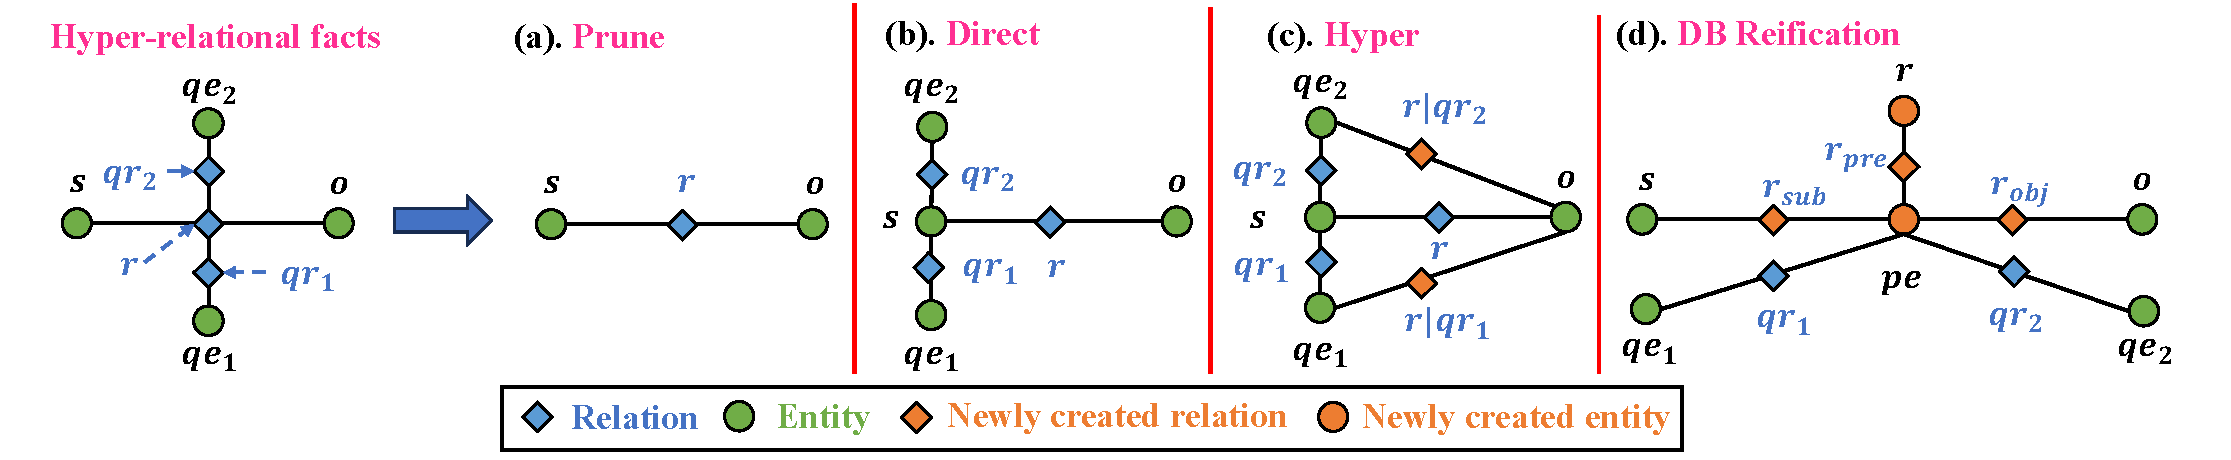
\includegraphics[width=\linewidth]{figures/hyperkg/decomp_new.pdf}
\caption{Original comparison of hyper-relational decomposition methods. Prune retains the main triple; Direct adds subject--qualifier links; Hyper adds combined relations; database reification introduces auxiliary objects. Reproduced from Fig.~1 of the CIKM study~\cite{bg-hyperkg}.}
\label{fig:background:decomposition}
\end{figure}

Qualifier associations matter when a subject participates in several facts with the same relation. For example, a degree qualifies a particular university attendance statement. Separate subject--degree and subject--university triples retain the entities but change how that association is represented. Hyper adds connections intended to preserve these associations. A qualifier integrator instead receives the main fact and its qualifier pairs together.

We compare conventional KGE models under these transformations with specialized HKGE models. Some GNN-based configurations obtain comparable scores on Cleaned JF17k and WD50k. Adding qualifier-derived edges changes the graph paths available to an encoder, so information preservation depends on both the transformed data and the model that processes it.

\subsection{Qualifier Capture and Graph Reception}

The analysis separates qualifier capture from graph reception. Qualifier capture concerns how the model represents qualifier pairs and their association with the main statement. Graph reception concerns how it receives information from the wider graph, including dependencies beyond one fact. Models operating on a fact in isolation have a different receptive field from graph encoders that propagate information across several hops. These properties are visible in the operations used to construct representations.

CompGCN jointly models entity and relation representations in a multi-relational graph~\cite{bg-compgcn}. NBFNet aggregates path information for link prediction~\cite{bg-nbfnet}. Their graph computations offer different ways to receive neighborhood and path information after decomposition. The CIKM analysis also identifies an information-compression issue when qualifier information is aggregated into fixed-size main-triple representations. Wider graph reception and qualifier integration consequently concern complementary parts of the architecture. The study evaluates designs that retain both sources for prediction.

FormerGNN combines a Transformer-based qualifier integrator operating on the original hyper-relational facts with a graph encoder operating on the pruned main-triple graph. The graph encoder generates a topology representation for the subject. The model concatenates this representation with representations of the main triple and qualifier pairs and passes them to a Transformer decoder. This organization supplies qualifier and graph information jointly to the prediction stage. In the reported configuration, HyperFormer provides the qualifier integrator and NBFNet provides the graph encoder~\cite{bg-hyperformer,bg-nbfnet}.

\subsection{Representative Published Evidence}

Table~\ref{tab:background:formergnn} reproduces the Cleaned JF17k and WD50k columns of the study's Table~6. MRR measures mean reciprocal rank, and H@1 and H@10 measure whether the target entity appears within the corresponding rank cutoff. These are link-prediction measures, distinct from the annotation and answer metrics of the later chapters.

\begin{table}[tbp]
\centering
\caption{Projection of the CIKM study's Table~6 onto Cleaned JF17k and WD50k. All model rows and the original metric precision are retained; the original bold and underline markings indicate best and second-best values.}
\label{tab:background:formergnn}
\small
\begin{tabular}{lrrrrrr}
\toprule
&\multicolumn{3}{c}{Cleaned JF17k}&\multicolumn{3}{c}{WD50k}\\
\cmidrule(lr){2-4}\cmidrule(lr){5-7}
Model&MRR&H@1&H@10&MRR&H@1&H@10\\
\midrule
StarE&0.381&0.284&0.577&0.346&0.268&0.494\\
QUAD&0.402&0.305&0.602&0.349&0.275&0.487\\
HAHE&0.405&0.310&0.585&0.360&0.288&0.496\\
HyperFormer&\underline{0.425}&\underline{0.328}&0.613&\underline{0.372}&\underline{0.293}&0.522\\
NBFNet + Prune&0.415&0.313&\textbf{0.630}&0.360&0.271&\textbf{0.530}\\
CompGCN + Hyper&0.389&0.294&0.590&0.350&0.277&0.488\\
FormerGNN&\textbf{0.432}&\textbf{0.335}&\underline{0.624}&\textbf{0.377}&\textbf{0.299}&\underline{0.527}\\
\bottomrule
\end{tabular}
\end{table}

FormerGNN obtains MRR 0.432 on Cleaned JF17k and 0.377 on WD50k, compared with HyperFormer's 0.425 and 0.372. NBFNet + Prune has the highest H@10 in both selected datasets, at 0.630 and 0.530. The experiment uses a single NVIDIA A100-40GB GPU. Parameters follow the original repositories or are selected by grid search when dataset-specific settings are unavailable. For comparisons involving CompGCN, the study replaces its decoder with a Transformer to align it with the corresponding HKGE configurations.

The complete comparison also includes Wikipeople and FBAUTO, with different dataset characteristics and metric rankings. The study shows how changing the organization of graph facts changes the information available to a prediction model.

\section{Research Questions Emerging from the Background}
\label{sec:background:questions}

Knowledge-enhanced annotation motivates our first question about supplying missing context and learning its correspondence to labels. Dependence on existing graphs and supervised training then motivates graph construction from task data and adaptation through retrieval. Extending retrieval beyond classification introduces questions about connected evidence and answer coverage for text, and query-aware construction and semantic matching for multimodal sources. The following chapters investigate these questions.
